\documentclass{article}
\usepackage[utf8]{inputenc}
\usepackage{amsmath,amsfonts,amssymb,amsthm}
\usepackage{graphicx}
\usepackage{url}
\usepackage{hyperref}
\usepackage{xcolor}
\usepackage{booktabs}
\usepackage{multirow}
\usepackage[margin=1in]{geometry}
\usepackage{float}

\newcommand{\software}[1]{\texttt{#1}}

\newtheorem{theorem}{Theorem}[section]
\newtheorem{proposition}{Proposition}[section]
\newtheorem{remark}{Remark}[section]

\title{PowerSim: A Simulation-Based Power Assessment Framework for Differential Circadian Rhythm Analysis}
\author{}
\date{}

\begin{document}

\maketitle

\begin{abstract}
Differential circadian rhythm analysis—comparing rhythmic gene expression between conditions—is central to understanding circadian disruption in disease, but no tools provide prospective power analysis of differential rhythmicity (DR) or differential phase (DP) tests. Existing analytical approaches assume a common effect size across genes, but transcriptomic signal-to-noise ratios ($r = A/\sigma$) vary over a 50-fold range, making single-$r$ power calculations unreliable. We present \software{PowerSim}, a semi-parametric simulation framework that extends PROPER's empirical-distribution approach to circadian differential analysis. Using pilot data from the human prefrontal cortex (19,998 genes, 62 samples), we simulate 5,000 genes across 50 replications under a passive (observational) design. Key findings: (1) DR overall (marginal) per-gene power averaged across non-null genes reaches only 30.5\% at $n=100$ per group (FDR 5\%), underscoring the need for prospective design in costly post-mortem studies; (2) stratified analysis reveals that overall (marginal) per-gene power conceals a 0--83\% range across effect-size strata, with genes at $r > 1.25$ reliably detected at $n=60$ while $r < 0.5$ genes remain poorly powered ($<5\%$) even at $n = 100$; (3) DP power saturates beyond 8-hour phase shifts due to the geometric limit of cosine separation; and (4) a case study comparing DiffCircaPipeline (LRT) and CircaCompare (Wald NLS)—the only two methods testing individual circadian parameters—shows complementary strengths: DCP uniquely supports DR testing with strict FDR control, while CircaCompare achieves higher DP power at the cost of inflated DP FDR (9--20\%) and $75\times$ longer runtime. Framework validity is confirmed through null-simulation Type~I error control, power monotonicity, and FDR calibration. \software{PowerSim} is available as an open-source R framework.
\end{abstract}

%% ====================================================================
\section{Introduction}
%% ====================================================================

Circadian rhythms—endogenous $\sim$24-hour oscillations in gene expression—play fundamental roles in physiology and disease \cite{takahashi2017transcriptional}. Differential circadian analysis, comparing rhythmic patterns between conditions (e.g., young vs.\ old, healthy vs.\ diseased), has revealed widespread disruption of temporal gene regulation in aging \cite{chen2016aging} and neuropsychiatric disorders. Because rhythmic transcription shapes metabolism, synaptic function, and immune signaling, misalignment has direct consequences for disease biology \cite{takahashi2017transcriptional,mure2018diurnal,chen2016aging}. However, researchers lack tools to determine appropriate sample sizes for these studies, leading to underpowered experiments or wasteful oversampling. The need for prospective power analysis is especially acute for \emph{passive} (observational) designs, such as post-mortem human brain studies, where samples are scarce, collection times cannot be controlled, and each additional subject represents months of tissue procurement effort. In these settings, committing to a study without power guidance risks years of work on an underpowered design \cite{zong2023circapower}.


\software{PROPER} \cite{wu2015proper} demonstrated that simulation-based power analysis with empirical parameter distributions provides more realistic guidance for high-throughput studies than analytical formulas. We extend this approach to circadian biology, introducing \software{PowerSim}, a semi-parametric framework that evaluates DR/DP operating characteristics under the full DCP pipeline (screening $\rightarrow$ DR test $\rightarrow$ post-hoc DP phase test). \software{PowerSim} stratifies targeted power by the signal-to-noise ratio $r = A/\sigma$ into 15 strata, exposing heterogeneity that overall (marginal) per-gene power can conceal, and supports both active (controlled-timepoint) and passive (observational) sampling designs; passive designs use pilot-derived TOD distributions to estimate the design factor.

\paragraph{Contributions.}
\begin{itemize}
\item We provide the first prospective power framework for differential circadian tests (DR/DP), with primary focus on passive designs and a unified extension to active designs.
\item We quantify and visualize targeted power stratified by signal-to-noise $r$, revealing heterogeneity masked by overall averages and enabling effect-size-aware study planning.
\item We enable method-agnostic comparisons of differential circadian pipelines under identical simulations, reporting targeted power and FDR trade-offs under the full DCP pipeline.
\end{itemize}

%% ====================================================================
\section{Methods}
%% ====================================================================

We evaluate how experimental design affects operating characteristics in
differential circadian analysis using a simulation-based framework. Because
differential circadian inference is multi-stage---rhythmicity screening,
followed by DR/DP testing and multiplicity adjustment---closed-form power
calculations are generally unavailable for the full analysis pipeline. We
therefore assess power and error control empirically under realistic design
settings using simulations calibrated to pilot data.

The framework has two components. First, we generate simulated circadian
datasets using flexible gene-level models calibrated to pilot data, preserving
effect-size heterogeneity, noise heterogeneity, and variation in rhythmicity
strength across genes. Second, we apply the full
\software{DiffCircaPipeline} (DCP) to each simulated dataset and summarize
operating characteristics across design scenarios. The simulation model and
evaluation procedure are modular, allowing alternative simulators or detection
methods to be paired with the same pipeline-level power assessment.

Rather than summarizing performance by a single overall power curve, we
emphasize prospective power evaluation across a grid of realistic scenarios
that vary sample size, sampling schedule, screening rules, and gene-filtering
settings. We also report conditional power summaries stratified by rhythmicity
strength, e.g.\ $r_{g,k}=A_{g,k}/\sigma_{g,k}$, which are often more
informative for design than a single marginal average to evaluate the trade-off. This strategy follows
the prospective simulation-based philosophy of \software{PROPER}
\cite{wu2015proper}.

% --------------------------------------------------------------------
\subsection{Notations and Terminology}
\label{sec:notation}

We index genes by $g=1,\ldots,G$, subjects by $i$, and groups by
$k\in\{1,2\}$. Time-of-day is denoted by $t\in[0,24)$ hours, with period
$\tau=24$ and angular frequency $\omega=2\pi/\tau$. Gene-level cosinor
parameters are mesor $\mu_{g,k}$, amplitude $A_{g,k}$, acrophase
$\phi_{g,k}$, and noise level $\sigma_{g,k}$, with signal-to-noise ratio
$r_{g,k}=A_{g,k}/\sigma_{g,k}$.

DR denotes differential rhythmicity, i.e.\ gain or loss of rhythmicity between
groups, and DP denotes differential phase, i.e.\ a phase shift between groups
among genes rhythmic in both groups. Empirical parameter distributions
estimated from pilot data are denoted by $\hat{F}_\mu$,
$\hat{F}_{\sigma,k}$, and $\hat{F}_{A,k}$, with $k\in\{1,2\}$ when two-group
pilot data are available. The time-of-day sampling distribution for passive
designs is denoted by $\hat{F}_{\mathrm{TOD},k}$; in the single-group pilot
case we use $\hat{F}_{\mathrm{TOD},1}=\hat{F}_{\mathrm{TOD},2}$.

For endpoint $E\in\{\mathrm{DR},\mathrm{DP}\}$, let $D_g^E\in\{0,1\}$
indicate discovery by the analysis pipeline, $z_g^E\in\{0,1\}$ indicate a
true differential gene, and $z_g^{*,E}\in\{0,1\}$ indicate a targeted
differential gene whose true effect exceeds a user-specified threshold.
In active designs, we distinguish the number of distinct time points $B$ and
the number of replicates per time point $m_b$, so that the total sample size
per group is $n=\sum_{b=1}^B m_b.$

% --------------------------------------------------------------------
\subsection{Cosinor Model and Hypothesis Tests}
\label{sec:cosinor_tests}

For group $k\in\{1,2\}$ and gene $g$, we use the cosinor model
\begin{equation}
y_{g,k,i}
=
\mu_{g,k}
+
A_{g,k}\cos\!\bigl(\omega(t_{k,i}-\phi_{g,k})\bigr)
+
\varepsilon_{g,k,i},
\qquad
\varepsilon_{g,k,i}\overset{\text{iid}}{\sim}N(0,\sigma_{g,k}^2).
\label{eq:cosinor_model}
\end{equation}
Rhythmicity within each group is assessed by testing
$H_0:A_{g,k}=0$ versus $H_1:A_{g,k}\neq 0$ using the standard $F$ statistic
\begin{equation}
F_{g,k}
=
\frac{(\mathrm{TSS}_{g,k}-\mathrm{RSS}_{g,k})/2}
{\mathrm{RSS}_{g,k}/(N_k-3)}
\sim F(2,N_k-3),
\label{eq:rhythm_f_test}
\end{equation}
where $\mathrm{RSS}_{g,k}=\sum_{i=1}^{N_k}(y_{g,k,i}-\hat y_{g,k,i})^2$ is the
residual sum of squares, $\mathrm{TSS}_{g,k}=\sum_{i=1}^{N_k}(y_{g,k,i}-\bar
y_{g,k})^2$ is the total sum of squares, $\hat y_{g,k,i}$ is the fitted value
under the cosinor model, $\bar y_{g,k}=N_k^{-1}\sum_{i=1}^{N_k} y_{g,k,i}$ is
the group mean, and $N_k$ denotes the sample size in group $k$.
At significance level $\alpha$, the null is rejected when
$F_{g,k}>F_{1-\alpha,\,2,\,N_k-3}$.

For genes rhythmic in at least one group, DCP characterizes rhythm fitness by
$R^2=1-\mathrm{RSS}/\mathrm{TSS}$ and tests
\begin{equation}
H_{0,R^2}: R_{g,1}^2 = R_{g,2}^2
\qquad \text{vs.} \qquad
H_{A,R^2}: R_{g,1}^2 \neq R_{g,2}^2,
\label{eq:dr_r2_hyp}
\end{equation}
using a likelihood ratio test on the SNR-parameterized model.
When the sampled time points are matched across groups, equality of $R^2$
corresponds to equality of signal-to-noise ratio $A/\sigma$, providing the
interpretive basis for DR testing in DCP.

For genes rhythmic in both groups, DCP uses a two-stage parameter framework.
The global joint test evaluates
\begin{equation}
H_{0,(A,\phi)}:\; A_{g,1}=A_{g,2}\ \text{and}\ \phi_{g,1}=\phi_{g,2}
\qquad \text{vs.} \qquad
H_{A,(A,\phi)}:\; \text{complement},
\label{eq:dp_hyp}
\end{equation}
followed by post-hoc amplitude and phase tests with \v{S}id\'{a}k adjustment.
In our pipeline, the DP endpoint is the post-hoc phase-only test, consistent
with DCP’s recommendation when phase is the sole parameter of interest.

Throughout, DCP is treated as the fixed downstream inference procedure used to
evaluate operating characteristics under candidate study designs.

% --------------------------------------------------------------------
\subsection{Design Theory for Active and Passive Circadian Sampling}
\label{sec:design_theory}

In this paper, an \emph{active} design denotes a study in which investigators
specify the sampling schedule, including the number and placement of collection
times and, if applicable, replicates per time point, whereas a \emph{passive}
design denotes a study in which collection times are not controlled by the
investigator and are instead determined by an empirical time-of-day distribution. To make the role of sampling schedules explicit, we use the linearized
first-harmonic representation of the cosinor model,
\begin{equation}
y_{g,k}(t)
=
\mu_{g,k}
+
\beta_{g,k,1}\cos(\omega t)
+
\beta_{g,k,2}\sin(\omega t)
+
\varepsilon_{g,k}(t),
\qquad
\varepsilon_{g,k}(t)\sim N(0,\sigma_{g,k}^2),
\label{eq:cosinor_linear}
\end{equation}
which is algebraically equivalent to \eqref{eq:cosinor_model} through
\begin{equation}
A_{g,k}=\sqrt{\beta_{g,k,1}^2+\beta_{g,k,2}^2},
\qquad
\phi_{g,k}=\operatorname{atan2}\!\left(\beta_{g,k,2},\beta_{g,k,1}\right).
\label{eq:beta_to_phase}
\end{equation}
This representation is used only for design reasoning; downstream inference
remains the DCP procedure described above.

Let the design have $B$ distinct sampling times $\{t_b\}_{b=1}^B$ with $m_b$
replicates at time $t_b$, satisfying $\sum_{b=1}^B m_b=n$. Define
$f(t)=\bigl(1,\cos(\omega t),\sin(\omega t)\bigr)^\top$, and let
$X\in\mathbb{R}^{n\times 3}$ be the design matrix whose rows are $f(t_b)^\top$,
repeated $m_b$ times for each sampling time $t_b$. Under the Gaussian linear
model, the Fisher information for $(\mu_{g,k},\beta_{g,k,1},\beta_{g,k,2})$ is
proportional to
\begin{equation}
I(\mathcal{D}) \propto X^\top X
=
\sum_{b=1}^B m_b\, f(t_b)f(t_b)^\top,
\label{eq:info_matrix}
\end{equation}
where $\mathcal{D}=\{(t_b,m_b)\}_{b=1}^B$ denotes the sampling design.
Equation~\eqref{eq:info_matrix} shows that replication increases information by
reweighting existing time points through $m_b$, whereas adding new sampling
times changes the harmonic basis represented in the design and can improve
parameter identifiability.

We first consider balanced active designs. Under equally spaced sampling times
$t_b=(b-1)\tau/B$ with $B\geq 3$ and common replication $m$ per time point, so
that $n=Bm$, each distinct time contributes
$m\,f(t_b)f(t_b)^\top$ to $X^\top X$, giving
\begin{equation}
X^\top X
=
m\sum_{b=1}^B
\begin{bmatrix}
1 \\
\cos(\omega t_b) \\
\sin(\omega t_b)
\end{bmatrix}
\begin{bmatrix}
1 & \cos(\omega t_b) & \sin(\omega t_b)
\end{bmatrix}.
\label{eq:xtx_expand}
\end{equation}
Expanding the outer product yields
\begin{equation}
X^\top X
=
m
\begin{pmatrix}
\sum_{b=1}^B 1 &
\sum_{b=1}^B \cos(\omega t_b) &
\sum_{b=1}^B \sin(\omega t_b) \\[6pt]
\sum_{b=1}^B \cos(\omega t_b) &
\sum_{b=1}^B \cos^2(\omega t_b) &
\sum_{b=1}^B \cos(\omega t_b)\sin(\omega t_b) \\[6pt]
\sum_{b=1}^B \sin(\omega t_b) &
\sum_{b=1}^B \cos(\omega t_b)\sin(\omega t_b) &
\sum_{b=1}^B \sin^2(\omega t_b)
\end{pmatrix}.
\label{eq:xtx_sumform}
\end{equation}
For equally spaced points over one full cycle, the first-harmonic basis
functions are orthogonal on the sampled grid:
$\sum_{b=1}^B \cos(\omega t_b)=0$,
$\sum_{b=1}^B \sin(\omega t_b)=0$,
$\sum_{b=1}^B \cos(\omega t_b)\sin(\omega t_b)=0$,
and
$\sum_{b=1}^B \cos^2(\omega t_b)=\sum_{b=1}^B \sin^2(\omega t_b)=B/2$.
Substituting these identities into \eqref{eq:xtx_sumform} gives
\begin{equation}
X^\top X
=
m
\begin{pmatrix}
B & 0 & 0 \\
0 & B/2 & 0 \\
0 & 0 & B/2
\end{pmatrix}
=
\operatorname{diag}(n,n/2,n/2),
\label{eq:xtx_balanced}
\end{equation}
since $n=Bm$.

For notational simplicity, we suppress gene and group indices in the following
derivation. For the global rhythmicity test
$H_0:\beta_1=\beta_2=0$ in the linearized cosinor model, the noncentrality
parameter is determined by the $(\beta_1,\beta_2)$ block of $X^\top X$. Using
\eqref{eq:xtx_balanced},
\begin{equation}
\lambda
=
\frac{1}{\sigma^2}
\begin{pmatrix}\beta_1 & \beta_2\end{pmatrix}
\begin{pmatrix} n/2 & 0 \\ 0 & n/2 \end{pmatrix}
\begin{pmatrix}\beta_1 \\ \beta_2\end{pmatrix}
=
\frac{n}{2\sigma^2}(\beta_1^2+\beta_2^2)
=
\frac{n}{2}\left(\frac{A}{\sigma}\right)^2,
\label{eq:ncp_active}
\end{equation}
where $A^2=\beta_1^2+\beta_2^2$. Thus, within this class of balanced equally
spaced designs, detection efficiency depends on the total sample size $n$, but
not separately on the number of distinct time points $B$ and the replication
level $m$.

\begin{proposition}[$B$-invariance for balanced active designs]
\label{prop:b_invariance}
Under the cosinor model \eqref{eq:cosinor_model} with independent subjects, for
an active design with $B\geq 3$ equally spaced time points and balanced
replication, first-harmonic efficiency depends on the total sample size $n$ but
not separately on $B$ and $m$. Equivalently, the design factor is constant,
$d(\phi)=1/2$, for all phases $\phi$.
\end{proposition}

\begin{proof}
Under balanced equally spaced sampling,
$X^\top X=\operatorname{diag}(n,n/2,n/2)$ by
\eqref{eq:xtx_balanced}, so the variances of $\hat\beta_1$ and $\hat\beta_2$
depend only on $n$. Moreover, the design factor
$d(\phi)=n^{-1}\sum_{i=1}^n \cos^2(\omega t_i-\omega\phi)$ reduces to $1/2$
uniformly in $\phi$ by the same orthogonality argument.
\end{proof}

Proposition~\ref{prop:b_invariance} provides the theoretical baseline for
balanced active designs: within this restricted class, reallocating effort
between the number of time points $B$ and replicates $m$ at fixed $n$ has
little effect on first-harmonic efficiency. This invariance breaks down when
sampling times are uneven or constrained, replication is unbalanced, repeated
measures induce correlation, or higher harmonics are relevant.

Passive circadian designs differ fundamentally because collection times are not
under investigator control. In passive datasets (e.g.\ post-mortem studies),
the sampled time-of-day distribution is generally uneven, so the design matrix
does not satisfy the orthogonality conditions above. In this case we write
$d(\phi)$ for the generic phase-dependent design factor and
$d_{g,k}=d(\phi_{g,k})$ for its value at gene-specific acrophase
$\phi_{g,k}$, with
\begin{equation}
d_{g,k}
=
\frac{1}{n_k}\sum_{i=1}^{n_k}
\cos^2\!\bigl(\omega t_{k,i}-\omega\phi_{g,k}\bigr).
\label{eq:design_factor}
\end{equation}
Thus $d_{g,k}$ varies across gene phase and group, implying that targeted power
and FDR depend jointly on sample size and time-of-day coverage. Genes peaking
in well-sampled windows receive larger effective information than genes peaking
in coverage gaps. For this reason, \software{PowerSim} reports design-factor
diagnostics in passive designs to quantify how temporal coverage alters
effective efficiency.

These considerations motivate two distinct design questions. In active designs,
the key issue is whether performance is driven mainly by total sample size or
also by the chosen number of time points. In passive designs, the central
question is how sample size and empirical time-of-day coverage jointly shape
detection performance. Both questions are addressed by the prospective
simulation framework described below.



% --------------------------------------------------------------------
\subsection{Study Design, Prospective Simulation, and Performance Metrics}
\label{sec:study_design}

We next formalize the study setting, simulation workflow, and performance
metrics used to evaluate prospective circadian study designs.

Consider a pilot circadian transcriptome dataset
\[
\mathcal{D}_0=
\Bigl\{
Y^{(0)}=\bigl(y^{(0)}_{g,i}\bigr)_{G_0\times N_0},
\;
t^{(0)}=\bigl(t_i^{(0)}\bigr)_{1\times N_0}
\Bigr\},
\]
where $y^{(0)}_{g,i}$ is the log-normalized expression of gene $g$ in pilot
subject $i$, and $t_i^{(0)}\in[0,24)$ is the collection time.
Based on $\mathcal{D}_0$, we study a future two-group experiment with $G$
genes, group index $k\in\{1,2\}$, and planned sample sizes $(n_1,n_2)$,
under either an active design (user-specified collection times) or a passive
design (collection times drawn from an empirical time-of-day distribution).
Throughout, we fix $\tau=24$\,h and $\omega=2\pi/\tau$.

The study setting is specified by the total number of genes $G$, group sample
sizes $(n_1,n_2)$, circadian period $\tau$, design type, simulation
hyperparameters
\[
\mathcal{H}
=
\{\pi_{\mathrm{DR}},\pi_{\mathrm{rhythmic}},\pi_{\mathrm{DP}},
\Delta\phi_{\min},\Delta\phi_{\max}\},
\]
analysis hyperparameters including the user-specified nominal FDR level
$\alpha$, and pilot-derived empirical distributions $\hat{F}_\mu$,
$\hat{F}_{\sigma,k}$, $\hat{F}_{A,k}$, and
$\hat{F}_{\mathrm{TOD},k}$ for $k\in\{1,2\}$.
Here $\pi_{\mathrm{DR}}$ denotes the proportion of DR genes,
$\pi_{\mathrm{rhythmic}}$ the proportion of non-DR genes that are jointly
rhythmic, and $\pi_{\mathrm{DP}}$ the proportion of genes assigned
differential phase. When only one-group pilot data are available, we use
$k=1$ distributions for both groups.

We denote the resulting study specification by
\[
\mathcal{S}
=
(G,n_1,n_2,\omega,\mathcal{H},\alpha,\hat{F}_\mu,
\hat{F}_{\sigma,k},\hat{F}_{A,k},\hat{F}_{\mathrm{TOD},k}),
\]
and condition on $\mathcal{S}$ implicitly.

Given $\mathcal{S}$, the \software{PowerSim} workflow proceeds in four stages.
First, gene-level cosinor models are fit to the pilot data to estimate
empirical parameter distributions. Second, two-group circadian expression data
are generated from a semi-parametric model parameterized by the pilot
estimates. Third, DCP is applied to each simulated dataset to obtain TOJR
labels and DR/DP $p$-values. Finally, targeted power and error rates are
aggregated across simulation replicates and signal-to-noise strata.

This prospective simulation framework also supports experimental-design
comparisons. For active designs, candidate schedules may vary in the number and
placement of time points and in the allocation of replication across them. For
passive designs, candidate scenarios vary sample size and the implied
time-of-day coverage through $\hat{F}_{\mathrm{TOD},k}$. In both cases,
operating characteristics are evaluated directly under the full downstream
pipeline rather than through a closed-form approximation.

To formalize operating characteristics, for each gene $g=1,\ldots,G$ and
endpoint $E\in\{\mathrm{DR},\mathrm{DP}\}$ let $D_g^E\in\{0,1\}$ indicate
discovery by the full DCP pipeline, $z_g^E\in\{0,1\}$ indicate a true
differential gene, and $z_g^{*,E}\in\{0,1\}$ indicate a biologically
meaningful differential effect above a user-defined threshold $\Delta$.
For each endpoint, operating characteristics are evaluated under the full DCP
pipeline, including rhythmicity screening, DR/DP testing, and BH correction at
nominal level $\alpha$.

Let $R^E=\sum_g D_g^E$ be the total number of discoveries,
$V^E=\sum_g D_g^E(1-z_g^E)$ the number of false discoveries, and
$G_0^E=\sum_g(1-z_g^E)$ the number of true null genes.
The empirical marginal type I error rate is
\[
\mathrm{TypeI}^E=\frac{V^E}{G_0^E},
\]
and the empirical marginal false discovery rate is
\[
\mathrm{FDR}^E=\frac{V^E}{R^E},
\]
which measures the false discovery proportion among detected genes under the
full pipeline.

Let $G_1^{*,E}=\sum_g z_g^{*,E}$ be the number of targeted non-null genes,
where $z_g^{*,E}=1$ indicates that gene $g$ has a true endpoint-specific effect
size at least $\Delta$, with $\Delta$ denoting a user-specified minimum
biologically meaningful effect size, and let
$S^{*,E}=\sum_g D_g^E z_g^{*,E}$ be the number of targeted discoveries.
The empirical marginal targeted power is
\begin{equation}
\mathrm{TPower}^E(\Delta)=\frac{S^{*,E}}{G_1^{*,E}}.
\label{eq:tpower_def}
\end{equation}
When $\Delta=0$, targeted power coincides with the usual average power over all
non-null genes. For $\Delta>0$, it quantifies genome-wide detection
performance for biologically meaningful effects under the full DCP pipeline and
serves as the primary criterion for design evaluation.

Let $W_g$ be a stratification variable and $\{B_j\}$ a set of bins, e.g.\
signal-to-noise ratio $r_{g,k}=A_{g,k}/\sigma_{g,k}$, phase $\phi_g$, design
efficiency $d_{g,k}$, or mean expression level. Stratified targeted power is
\begin{equation}
\mathrm{TPower}_j^E(\Delta)
=
\frac{\sum_{g:W_g\in B_j} D_g^E z_g^{*,E}}
{\sum_{g:W_g\in B_j} z_g^{*,E}},
\label{eq:tpower_strat_def}
\end{equation}
which identifies regimes where a design is underpowered and informs analysis
planning.

To emphasize the prospective design perspective, operating characteristics are
summarized in several complementary ways, including marginal targeted power and
marginal FDR as functions of $n$, stratified targeted power by signal-to-noise
ratio, discovery-yield summaries such as $\mathbb{E}[R^E]$, and
design-efficiency diagnostics for passive sampling designs.

% --------------------------------------------------------------------
\subsection{Step I: Pilot Parameter Estimation}
\label{sec:pilot}

For each of the $G_0$ genes in the pilot dataset, we fit the linearized cosinor
model by ordinary least squares:
\begin{equation}
y_g^{(0)}=\mu_g\mathbf{1}+E_g\mathbf{c}+F_g\mathbf{s}+\boldsymbol\varepsilon_g,
\qquad
\mathbf{c}_i=\cos(\omega t_i^{(0)}),\;\mathbf{s}_i=\sin(\omega t_i^{(0)}),
\label{eq:pilot_fit}
\end{equation}
yielding estimates $\hat{\mu}_g$, $\hat{E}_g$, and $\hat{F}_g$.
Amplitude and acrophase are recovered as
\[
\hat{A}_g=\sqrt{\hat{E}_g^2+\hat{F}_g^2},
\qquad
\hat{\phi}_g=\frac{1}{\omega}\,\mathrm{atan2}\!\left(\hat{F}_g,\hat{E}_g\right),
\]
and the noise level is estimated by the MLE residual standard deviation
\begin{equation}
\hat{\sigma}_g
=
\left[
\frac{1}{N_0}\sum_{i=1}^{N_0}
\bigl(
y_{g,i}^{(0)}-\hat{\mu}_g-\hat{A}_g\cos(\omega t_i^{(0)}-\omega\hat{\phi}_g)
\bigr)^2
\right]^{1/2}.
\label{eq:pilot_sigma}
\end{equation}
A BH-adjusted rhythmicity $q$-value for $H_0:E_g=F_g=0$ is obtained from the
OLS $F$-test, and the rhythmic gene set is defined as
$\mathcal{G}_R=\{g:q_g<0.10\}$.

From the pilot data, we construct empirical distributions
\begin{equation}
\hat{F}_\mu=\frac{1}{G_0}\sum_{g=1}^{G_0}\delta_{\hat{\mu}_g},
\quad
\hat{F}_{\sigma,1}=\frac{1}{G_0}\sum_{g=1}^{G_0}\delta_{\hat{\sigma}_g},
\quad
\hat{F}_{A,1}=\frac{1}{|\mathcal{G}_R|}\sum_{g\in\mathcal{G}_R}\delta_{\hat{A}_g},
\label{eq:empirical_dists}
\end{equation}
where $\hat{F}_\mu$ and $\hat{F}_{\sigma,1}$ are estimated from all genes, but
$\hat{F}_{A,1}$ is restricted to rhythmic genes. Sampling from these empirical
distributions means drawing with replacement from the corresponding estimated
gene-level quantities.

When two-group pilot data are available,
\texttt{estCircadianParamTwoGroup()} additionally estimates
$\hat{F}_{\sigma,2}$, $\hat{F}_{A,2}$, and $\hat{F}_{\mathrm{TOD},2}$ from
group 2. It also estimates differential simulation hyperparameters
$(\pi_{\mathrm{DR}},\pi_{\mathrm{DP}},\Delta\phi_{\min},\Delta\phi_{\max})$
empirically by fitting cosinor models in each group and summarizing
cross-group rhythmicity and phase differences. In particular,
$\hat{\pi}_{\mathrm{DR}}$ is the proportion of genes rhythmic in exactly one
group, $\hat{\pi}_{\mathrm{DP}}$ is the proportion of jointly rhythmic genes
with phase shift exceeding a default threshold, and
$[\Delta\phi_{\min},\Delta\phi_{\max}]$ is taken from the empirical range or
interquartile range of the observed phase shifts. The function returns a fully
populated \texttt{CircadianBioOptions} object and associated diagnostics for use
in the simulation step.

% --------------------------------------------------------------------
\subsection{Step II: Data Generation Under a Circadian Model}
\label{sec:generative}

In Step~II, we generate a two-group dataset by drawing baseline parameters,
assigning each gene to a differential type, translating the type into
group-specific rhythmic parameters, sampling subject collection times, and
generating observations with Gaussian noise.

For $g=1,\ldots,G$, draw independently
\begin{equation}
\mu_g \overset{\mathrm{iid}}{\sim}\hat{F}_\mu,\quad
\sigma_{g,1} \overset{\mathrm{iid}}{\sim}\hat{F}_{\sigma,1},\quad
A_g \overset{\mathrm{iid}}{\sim}\hat{F}_{A,1}\text{ subject to }A_g\geq 0.05,\quad
\phi_g \overset{\mathrm{iid}}{\sim}\mathrm{Unif}(0,24).
\label{eq:layer1}
\end{equation}
The phase is drawn uniformly to avoid imposing a preferred peak time, and the
amplitude floor prevents degenerate near-zero oscillations that destabilize
phase estimation.

Gene types are assigned sequentially to preserve the pool structure required by
the downstream DP test. We use labels $T_g=0$ (arrhythmic in both groups),
$T_g=1$ (jointly rhythmic), $T_g=2$ (DR: rhythmic in group 1 only),
$T_g=3$ (DR: rhythmic in group 2 only), and $T_g=4$ (DP). Let
$\mathcal{A}=\{1,\ldots,G\}$.

\begin{enumerate}
\item Draw $n_{\mathrm{DR}}=\lfloor\pi_{\mathrm{DR}}G\rfloor$ genes uniformly
without replacement from $\mathcal{A}$. Assign the first
$\lceil n_{\mathrm{DR}}/2\rceil$ genes type $T_g=2$ and the remainder type
$T_g=3$.
\item From the non-DR remainder, draw
$\lfloor\pi_{\mathrm{rhythmic}}|\mathcal{A}\setminus\mathcal{G}_{\mathrm{DR}}|\rfloor$
genes to form the jointly rhythmic pool $\mathcal{J}$.
\item Draw $n_{\mathrm{DP}}=\lfloor\pi_{\mathrm{DP}}G\rfloor$ genes from
$\mathcal{J}$ and assign them type
$T_g=4$.
\item Assign the remaining genes in $\mathcal{J}$ type $T_g=1$ and all others
type $T_g=0$.
\end{enumerate}

This hierarchy ensures that DP genes are a subset of the jointly rhythmic pool,
as required by the DP detection step.

For type $T_g=3$, we draw a fresh amplitude and phase for group 2:
\begin{equation}
A_g^* \mid (T_g=3)\overset{\mathrm{iid}}{\sim}\hat{F}_{A,2}
\text{ subject to }A_g^*\geq 0.05,
\qquad
\phi_g^* \mid (T_g=3)\overset{\mathrm{iid}}{\sim}\mathrm{Unif}(0,24).
\label{eq:layer3a}
\end{equation}


For type $T_g=4$, we draw a phase shift
\begin{equation}
\Delta\phi_g\mid(T_g=4)\overset{\mathrm{iid}}{\sim}
\mathrm{Unif}(\Delta\phi_{\min},\Delta\phi_{\max}).
\label{eq:layer3b}
\end{equation}


The resulting group-specific rhythm parameters are summarized in
Table~\ref{tab:type_mapping}.

\begin{table}[H]
\centering
\small
\begin{tabular}{c|ccccc}
\toprule
 & 0 (arrhy) & 1 (both) & 2 (g1-only) & 3 (g2-only) & 4 (DP) \\
\midrule
Group 1 $(A_{g,1},\phi_{g,1})$
& ( -- , -- )
& ( $A_g$, $\phi_g$ )
& ( $A_g$, $\phi_g$ )
& ( -- , -- )
& ( $A_g$, $\phi_g$ ) \\

Group 2 $(A_{g,2},\phi_{g,2})$
& ( -- , -- )
& ( $A_g$, $\phi_g$ )
& ( -- , -- )
& ( $A_g^*$, $\phi_g^*$ )
& ( $A_g$, $(\phi_g+\Delta\phi_g)\bmod 24$ ) \\
\bottomrule
\end{tabular}
\caption{Mapping between gene type $T_g$ and group-specific rhythm parameters.
Dashes indicate that amplitude and phase are undefined in the arrhythmic group.}
\label{tab:type_mapping}
\end{table}

We set $\mu_{g,1}=\mu_{g,2}=\mu_g$ so that power comparisons isolate rhythmic
differences rather than baseline shifts. Noise is generated as
\begin{equation}
\sigma_{g,k}\overset{\mathrm{iid}}{\sim}\hat{F}_{\sigma,k},
\qquad k=1,2,
\label{eq:noise_gen}
\end{equation}
with $\hat{F}_{\sigma,2}=\hat{F}_{\sigma,1}$ in the single-group pilot case.

For DR genes, the relevant effect size is the SNR of the rhythmic group. For
DP genes, the relevant phase-separation effect size is controlled by
$\Delta\phi_g$, with effective contrast depending on both SNR and phase shift.

Collection times are generated according to the design type. For passive
designs,
\begin{equation}
t_{k,i}\overset{\mathrm{iid}}{\sim}\hat{F}_{\mathrm{TOD},k}
\text{ on }[0,24),
\qquad i=1,\ldots,n_k,\ k=1,2.
\label{eq:passive_times}
\end{equation}
For active designs, the user specifies a schedule through the number and
placement of time points and their replication counts. A balanced equally
spaced design corresponds to
\begin{equation}
c_b = \frac{(b-1)\tau}{B},\qquad b=1,\ldots,B,
\label{eq:active_bins}
\end{equation}
with replication allocated across bins through $\{m_b\}_{b=1}^B$.
This setup allows \software{PowerSim} to explore the trade-off between total
sample size $n$, the number of distinct time points $B$, and replication
allocation under controlled active sampling.

Conditional on all preceding steps, observations are generated as
\begin{equation}
y_{g,k,i}
=
\mu_g
+
A_{g,k}\cos(\omega t_{k,i}-\omega\phi_{g,k})
+
\varepsilon_{g,k,i},
\qquad
\varepsilon_{g,k,i}\overset{\mathrm{iid}}{\sim}N(0,\sigma_{g,k}^2).
\label{eq:obs}
\end{equation}

% --------------------------------------------------------------------
\subsection{Step III: Detection via DiffCircaPipeline}
\label{sec:dcp}

Given a simulated dataset $\{y_{g,k,i},t_{k,i}\}$, DCP estimates
group-specific parameters and performs differential circadian inference in
three stages.

First, for each group $k\in\{1,2\}$, DCP fits the linearized cosinor model
\[
y_{g,k,i}
=
\mu_{g,k}
+
E_{g,k}\cos(\omega t_{k,i})
+
F_{g,k}\sin(\omega t_{k,i})
+
\varepsilon_{g,k,i}
\]
jointly across all genes using \software{limma}'s \texttt{lmFit}
\cite{smyth2004linear}, followed by empirical Bayes variance moderation with
\texttt{eBayes(trend=TRUE, robust=TRUE)}. An $F$-test on
$(E_{g,k},F_{g,k})$ yields a raw rhythmicity $p$-value $p_{g,k}$ for each
gene and group.

Second, the Type of Joint Rhythmicity (TOJR) classifier assigns
\begin{equation}
\hat{Z}_g =
\begin{cases}
\texttt{arrhy} & p_{g,1}>\alpha \text{ and } p_{g,2}>\alpha,\\
\texttt{g1-only} & p_{g,1}\leq\alpha \text{ and } p_{g,2}>\alpha,\\
\texttt{g2-only} & p_{g,1}>\alpha \text{ and } p_{g,2}\leq\alpha,\\
\texttt{both} & p_{g,1}\leq\alpha \text{ and } p_{g,2}\leq\alpha,
\end{cases}
\label{eq:tojr}
\end{equation}
using unadjusted group-specific rhythmicity $p$-values.

Third, DR and DP testing are performed conditionally on the TOJR class. For
all genes with $\hat{Z}_g\neq\texttt{arrhy}$, DCP tests
$H_0:R^2_{g,1}=R^2_{g,2}$ by a $\Delta R^2$ likelihood ratio test
\cite{ding2021likelihood}, followed by BH correction across the tested genes.
Genes not entering the DR stage are assigned $p_g^{\mathrm{DR}}=1$.
For genes with $\hat{Z}_g=\texttt{both}$, DCP uses the two-stage parameter
framework described above; in our pipeline, the DP endpoint is the post-hoc
phase-only test, and BH correction is applied within the jointly rhythmic
stratum. Genes outside that stratum are assigned $p_g^{\mathrm{DP}}=1$.

% --------------------------------------------------------------------
\subsection{Step IV: Power and FDR Metrics}
\label{sec:metrics}

For each endpoint $E\in\{\mathrm{DR},\mathrm{DP}\}$, the ground-truth
differential indicator $z_g^E$ and targeted indicator $z_g^{*,E}$ are defined
from the simulated gene type and its true effect size.

For DR,
\begin{equation}
z_g^{\mathrm{DR}} = \mathbf{1}\{T_g\in\{2,3\}\},
\qquad
z_g^{*,\mathrm{DR}}
=
z_g^{\mathrm{DR}}
\cdot
\mathbf{1}\!\left\{
\frac{\max(A_{g,1},A_{g,2})}{\sigma_{g,\mathrm{rhythmic}}}\geq\delta^*
\right\},
\label{eq:dr_target}
\end{equation}
where $\sigma_{g,\mathrm{rhythmic}}$ is the noise level of the rhythmic group.

For DP,
\begin{equation}
z_g^{\mathrm{DP}} = \mathbf{1}\{T_g=4\},
\end{equation}
and the natural phase-separation effect size is
\begin{equation}
r_g^{\mathrm{DP}}
=
\frac{\sqrt{A_{g,1}^2+A_{g,2}^2-2A_{g,1}A_{g,2}\cos(\omega\Delta\phi_g)}}{\sigma_{g,1}}
=
2r_g\left|\sin\!\left(\frac{\pi\Delta\phi_g}{24}\right)\right|,
\label{eq:dp_snr}
\end{equation}
so that
\begin{equation}
z_g^{*,\mathrm{DP}}
=
z_g^{\mathrm{DP}}\cdot
\mathbf{1}\!\left\{r_g^{\mathrm{DP}}\geq\delta^*\right\}.
\label{eq:dp_target}
\end{equation}

For a given test $E$, let $D_g^E\in\{0,1\}$ indicate rejection after BH
correction at level $\alpha=0.05$. For simulation replicate $s$, the
per-replicate estimates
\[
\widehat{\mathrm{TPower}}_s^{E}
=
\frac{\sum_g D_g^{E} z_g^{*,E}}{\sum_g z_g^{*,E}},
\qquad
\widehat{\mathrm{FDR}}_s^{E}
=
\frac{\sum_g D_g^{E}(1-z_g^{E})}{\sum_g D_g^{E}}
\cdot\mathbf{1}\!\left\{\sum_g D_g^{E}>0\right\}
\]
are averaged over replicates to estimate marginal targeted power and marginal
FDR.

To characterize heterogeneity in detectability, genes are stratified by
signal-to-noise ratio. For DR, the stratification variable is the SNR of the
rhythmic group. For DP, we use either the effective phase-separation quantity
$r_g^{\mathrm{DP}}$ or a related SNR proxy, depending on the analysis. Stratum-level
targeted power is computed analogously to \eqref{eq:tpower_def}, with the
sums restricted to genes within each bin.

\software{PowerSim} also supports alternative detection backends such as
\software{CircaCompare} \cite{parsons2020circacompare}. Running multiple
methods on identical simulated datasets enables direct power--FDR comparisons
without confounding from data variability.

% --------------------------------------------------------------------
\subsection{Two-Stage (Plug-In) Power Analysis}
\label{sec:two_stage}

The prospective power analysis described in Steps~I--IV constitutes a
\emph{two-stage plug-in} procedure. In Stage~1, Step~I is applied once to
the pilot data $\mathcal{D}_0$, yielding single point estimates
$(\hat{\pi}_{\mathrm{DR}},\hat{F}_{A,k},\hat{F}_{\sigma,k})$. In Stage~2,
Steps~II--IV are executed at each candidate sample size $n$ in a design grid,
treating the Stage-1 estimates as fixed population quantities. The resulting
power curve
\begin{equation}
\widehat{\mathrm{Power}}_{\mathrm{TS}}(n)
=
\frac{1}{S}\sum_{s=1}^{S}\widehat{\mathrm{TPower}}_s^{E}(n)
\label{eq:two_stage_power}
\end{equation}
is a deterministic function of the pilot, and the minimum-sample-size
recommendation $\hat{n}_{80}=\min\!\bigl\{n:\widehat{\mathrm{Power}}_{\mathrm{TS}}(n)\geq 0.80\bigr\}$
carries no uncertainty quantification. Because the Stage-1 estimates are
treated as exact, estimation error in $\hat{\pi}_{\mathrm{DR}}$, $\hat{F}_{A,k}$,
or $\hat{F}_{\sigma,k}$ propagates directly into the power projection without
acknowledgement, typically yielding overoptimistic recommendations when the
pilot sample is small.

% --------------------------------------------------------------------
\subsection{Bootstrap-Based Design Grid}
\label{sec:bootstrap}

To propagate pilot uncertainty into the prospective power estimate, we replace
the single pilot fit in Stage~1 with a nonparametric bootstrap. Let the pilot
dataset contain $N_0$ subjects. For each bootstrap replicate $b=1,\ldots,B_{\mathrm{boot}}$:

\begin{enumerate}
\item Draw $N_0$ subjects with replacement from $\mathcal{D}_0$ to form
bootstrap resample $\mathcal{D}_0^{(b)}$.

\item Apply Step~I to $\mathcal{D}_0^{(b)}$ to obtain bootstrap parameter
estimates
\[
\bigl(\hat{\pi}_{\mathrm{DR}}^{(b)},\;\hat{F}_{A,k}^{(b)},\;\hat{F}_{\sigma,k}^{(b)}\bigr).
\]

\item For each candidate design $(n,B)$ in the evaluation grid, run Steps~II--IV
with the bootstrap estimates as inputs over $S_{\mathrm{inner}}$ simulation
replicates, yielding bootstrap power
\begin{equation}
\widehat{\mathrm{Power}}^{(b)}(n,B)
=
\frac{1}{S_{\mathrm{inner}}}
\sum_{s=1}^{S_{\mathrm{inner}}}
\widehat{\mathrm{TPower}}_s^{E,(b)}(n,B).
\label{eq:boot_power_rep}
\end{equation}
\end{enumerate}

Across the $B_{\mathrm{boot}}$ replicates, the bootstrap mean power at each
design point $(n,B)$ is
\begin{equation}
\bar{P}(n,B)
=
\frac{1}{B_{\mathrm{boot}}}
\sum_{b=1}^{B_{\mathrm{boot}}}
\widehat{\mathrm{Power}}^{(b)}(n,B),
\label{eq:boot_mean}
\end{equation}
and a $(1-\alpha_{\mathrm{CI}})$ bootstrap confidence interval is formed from
the empirical quantiles of the resample distribution,
\begin{equation}
\mathrm{CI}(n,B)
=
\bigl[
\widehat{\mathrm{Power}}_{\,\alpha_{\mathrm{CI}}/2}(n,B),\;
\widehat{\mathrm{Power}}_{\,1-\alpha_{\mathrm{CI}}/2}(n,B)
\bigr],
\label{eq:boot_ci}
\end{equation}
where $\widehat{\mathrm{Power}}_q(n,B)$ denotes the $q$-th empirical quantile
of $\bigl\{\widehat{\mathrm{Power}}^{(b)}(n,B)\bigr\}_{b=1}^{B_{\mathrm{boot}}}$.

The interval \eqref{eq:boot_ci} reflects how sensitive the power projection
is to the specific composition of the pilot: a narrow interval indicates that
the pilot is sufficiently informative to pin down the operating characteristic,
whereas a wide interval reveals that the two-stage point estimate has false
precision. In expectation, the bootstrap mean \eqref{eq:boot_mean} approximates
the two-stage estimate \eqref{eq:two_stage_power}, but the resampling additionally
reveals the sampling variability that the plug-in approach suppresses.

Evaluating the design grid simultaneously across multiple values of $B$
addresses the allocation question of how to divide a fixed subject budget $n$
between distinct time points $B$ and replication $m=n/B$. For each $B$, the
bootstrap procedure yields a separate power curve $\bar{P}(\,\cdot\,,B)$ with
pointwise confidence intervals \eqref{eq:boot_ci}, enabling a direct empirical
comparison of design strategies. Comparing these curves identifies whether
increasing temporal coverage or replication more efficiently improves power
under the empirical parameter distributions estimated from the pilot, and
provides an empirical check of the $B$-invariance property stated in
Proposition~\ref{prop:b_invariance} under real data heterogeneity.


%% ====================================================================
\section{Results}
%% ====================================================================

\subsection{Pilot Data and Simulation Setup}

Parameters were estimated from human prefrontal cortex expression data (PFC younger group: BA11 + BA47 regions; 19,998 genes, 62 samples) \cite{chen2016aging}. Of 19,998 genes, 3,952 (19.8\%) passed the rhythmicity filter. Estimated parameters: mesor $5.17 \pm 1.83$, amplitude $0.126 \pm 0.065$, noise $\sigma = 0.213 \pm 0.072$, median $r = 0.556$, circular phase mean 12.1\,h. Here the median $r$ ($\tilde{r} = 0.556$) is computed across all rhythmic (filter-passing) genes rather than only top-ranked genes, which yields lower values than summaries based on the most significant genes; this choice captures the full effect-size distribution and yields conservative power estimates. All simulations use $G = 5{,}000$ genes, $N_{\text{sim}} = 50$, passive design with empirical collection times, $n \in \{20, 40, 60, 80, 100\}$ per group, and BH-adjusted FDR control.

To contextualize these effect sizes, Table~\ref{tab:effect_sizes} compares intrinsic effect sizes across publicly available circadian transcriptomic datasets (adapted from \cite{zong2023circapower}). Human post-mortem brain tissues consistently show low effect sizes (median core-gene $r = 0.71$--$1.04$), while actively-designed mouse studies yield substantially higher values ($r = 1.27$--$6.33$). 

\begin{table}[H]
\centering
\small
\begin{tabular}{ll|lrcc}
\toprule
Organism & Study & Tissue & $n$ & \multicolumn{1}{c}{Median $r$} & \multicolumn{1}{c}{Min $r$} \\
 & & & & \multicolumn{1}{c}{(7 core)} & \multicolumn{1}{c}{(top 100)} \\
\midrule
\multirow{6}{*}{\textit{H.\ sapiens}} & \multirow{2}{*}{Chen et al.\ \cite{chen2016aging}} & PFC (BA11) & 147 & 0.91 & 0.46 \\
 & & PFC (BA47) & 147 & 0.77 & 0.44 \\
 & \multirow{2}{*}{Ketchesin et al.\ \cite{ketchesin2021diurnal}} & Striatum (NAc) & 59 & 0.71 & 1.06 \\
 & & Striatum (caudate) & 59 & 1.04 & 0.82 \\
 & Seney et al.\ \cite{seney2019diurnal} & PFC & 104 & 0.79 & 0.55 \\

\midrule
\multirow{6}{*}{\textit{M.\ musculus}} & Hughes et al.\ \cite{hughes2009harmonics} & Liver & 48 & 2.00 & 2.77 \\
 & Gerstner et al.\ \cite{gerstner2016removal} & Cerebral cortex & 34 & 2.46 & 2.18 \\
 & Na et al.\ \cite{na2009comprehensive} & Liver & 36 & 3.65 & 3.69 \\
 & \multirow{3}{*}{Zhang et al.\ \cite{zhang2014comprehensive}} & Liver (GSE54650) & 24 & 3.51 & 3.67 \\
 & & Kidney & 24 & 6.33 & 3.65 \\
 & & Cerebellum & 24 & 3.52 & 2.01 \\
\bottomrule
\end{tabular}
\caption{Intrinsic effect sizes ($r = A/\sigma$) from public circadian transcriptomic datasets, adapted from \cite{zong2023circapower}. Effect sizes are estimated using the cosinor method: ``Median $r$ (7 core)'' is the median $r$ of 7 core circadian genes; ``Min $r$ (top 100)'' is the minimum $r$ among the top 100 significant genes. Human passive studies show $r \approx 0.6$--$1.0$; mouse active studies show $r \approx 2$--$6$. Our pipeline reports median $r$ across all rhythmic genes, which is expected to be lower than top-ranked summaries.}
\label{tab:effect_sizes}
\end{table}

\subsection{Differential Rhythmicity Power}

DR power was evaluated with 15\% of genes showing gain/loss of rhythm. Overall (marginal) per-gene power averages over all target genes and thus reflects the full $r$ distribution. At FDR 5\%, overall (marginal) per-gene power ranges from 1.1\% ($n = 20$) to 30.5\% ($n = 100$), with empirical FDR well controlled (0.018--0.028; Table~\ref{tab:main_power}). The low overall (marginal) per-gene power reflects the predominance of low-$r$ genes in human brain tissue, consistent with the low-end effect sizes in Table~\ref{tab:effect_sizes}. Stratified analysis (Figure~\ref{fig:dr_power}) reveals that genes with $r > 1.25$ achieve $\geq$83\% power at $n = 60$, while genes with $r < 0.5$ remain below 5\% power even at $n = 100$. Panel E shows that true discoveries are concentrated in higher-$r$ strata, and panel F shows the empirical distribution of DR targets across $r$ strata. Sensitivity to the nominal FDR threshold is shown in Figure~\ref{fig:dr_power}B,D.

\subsection{Differential Phase Power}

DP was evaluated with 15\% phase-shifted genes ($\pm$6\,h uniform). Marginal power averages over all target genes and thus reflects the full $r$ distribution. Marginal power reaches 68.7\% at $n = 100$ (Table~\ref{tab:main_power}), substantially higher than DR because phase-shifted genes retain rhythmicity in both groups. In the extended analysis (Figure~\ref{fig:dp_power}, panel C), marginal DP power exceeds 80\% at $n = 160$, indicating that DP becomes well powered at modestly larger sample sizes. Genes with $r > 0.75$ achieve $\geq$92\% power at $n = 60$ (Figure~\ref{fig:dp_power}). Panel E shows that true discoveries concentrate in moderate-to-high $r$ bins, and panel F shows the empirical distribution of DP targets across $r$ strata. Sensitivity to the nominal FDR threshold is shown in Figure~\ref{fig:dp_power}B,D.

\begin{table}[H]
\centering
\small
\begin{tabular}{r|rr|rr|rr}
\toprule
& \multicolumn{2}{c|}{FDR 5\%} & \multicolumn{2}{c|}{Emp.\ FDR} & \multicolumn{2}{c}{Avg TD} \\
$n$ & DR & DP & DR & DP & DR & DP \\
\midrule
20  & 1.1\%  & 13.3\% & 0.028 & 0.063 & 8   & 99  \\
40  & 5.4\%  & 34.5\% & 0.018 & 0.031 & 40  & 259 \\
60  & 13.1\% & 50.1\% & 0.020 & 0.024 & 98  & 376 \\
80  & 22.4\% & 61.4\% & 0.025 & 0.020 & 168 & 460 \\
100 & 30.5\% & 68.7\% & 0.021 & 0.023 & 229 & 515 \\
\bottomrule
\end{tabular}
\caption{Marginal power, empirical FDR, and average true discoveries for DR and DP tests (5,000 genes, 50 simulations, DCP method). Detailed results with standard errors in Supplementary Section~S1.}
\label{tab:main_power}
\end{table}

\begin{figure}[H]
\centering
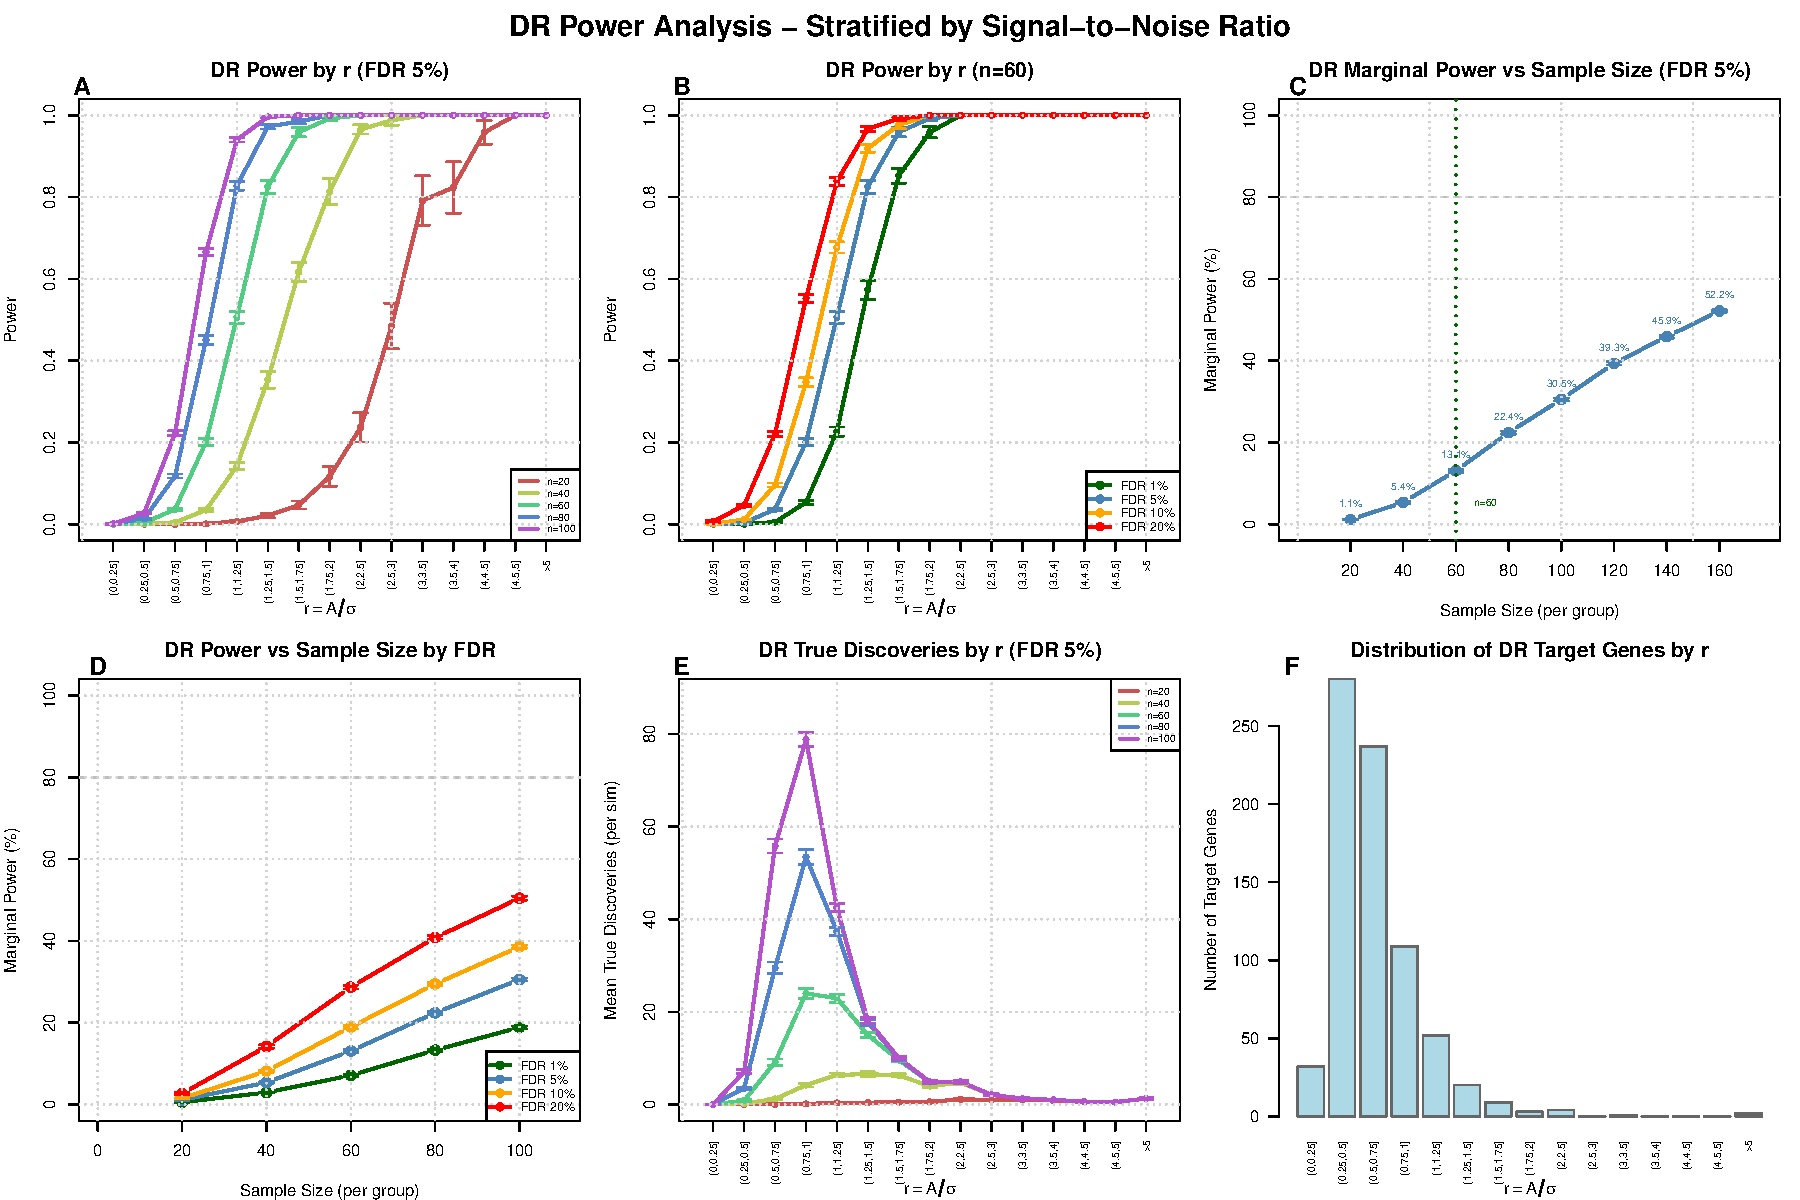
\includegraphics[width=\textwidth]{figures/dr_power.pdf}
\caption{DR power analysis. (A) Power by $r$ stratum at FDR 5\%. (B) Power by FDR threshold ($n=60$; sensitivity to nominal FDR). (C) Overall (marginal) per-gene power vs.\ sample size. (D) Overall (marginal) per-gene power by FDR threshold (sensitivity to nominal FDR). (E) True discoveries by $r$ stratum. (F) Empirical distribution of DR targets across $r$ strata.}
\label{fig:dr_power}
\end{figure}

\begin{figure}[H]
\centering
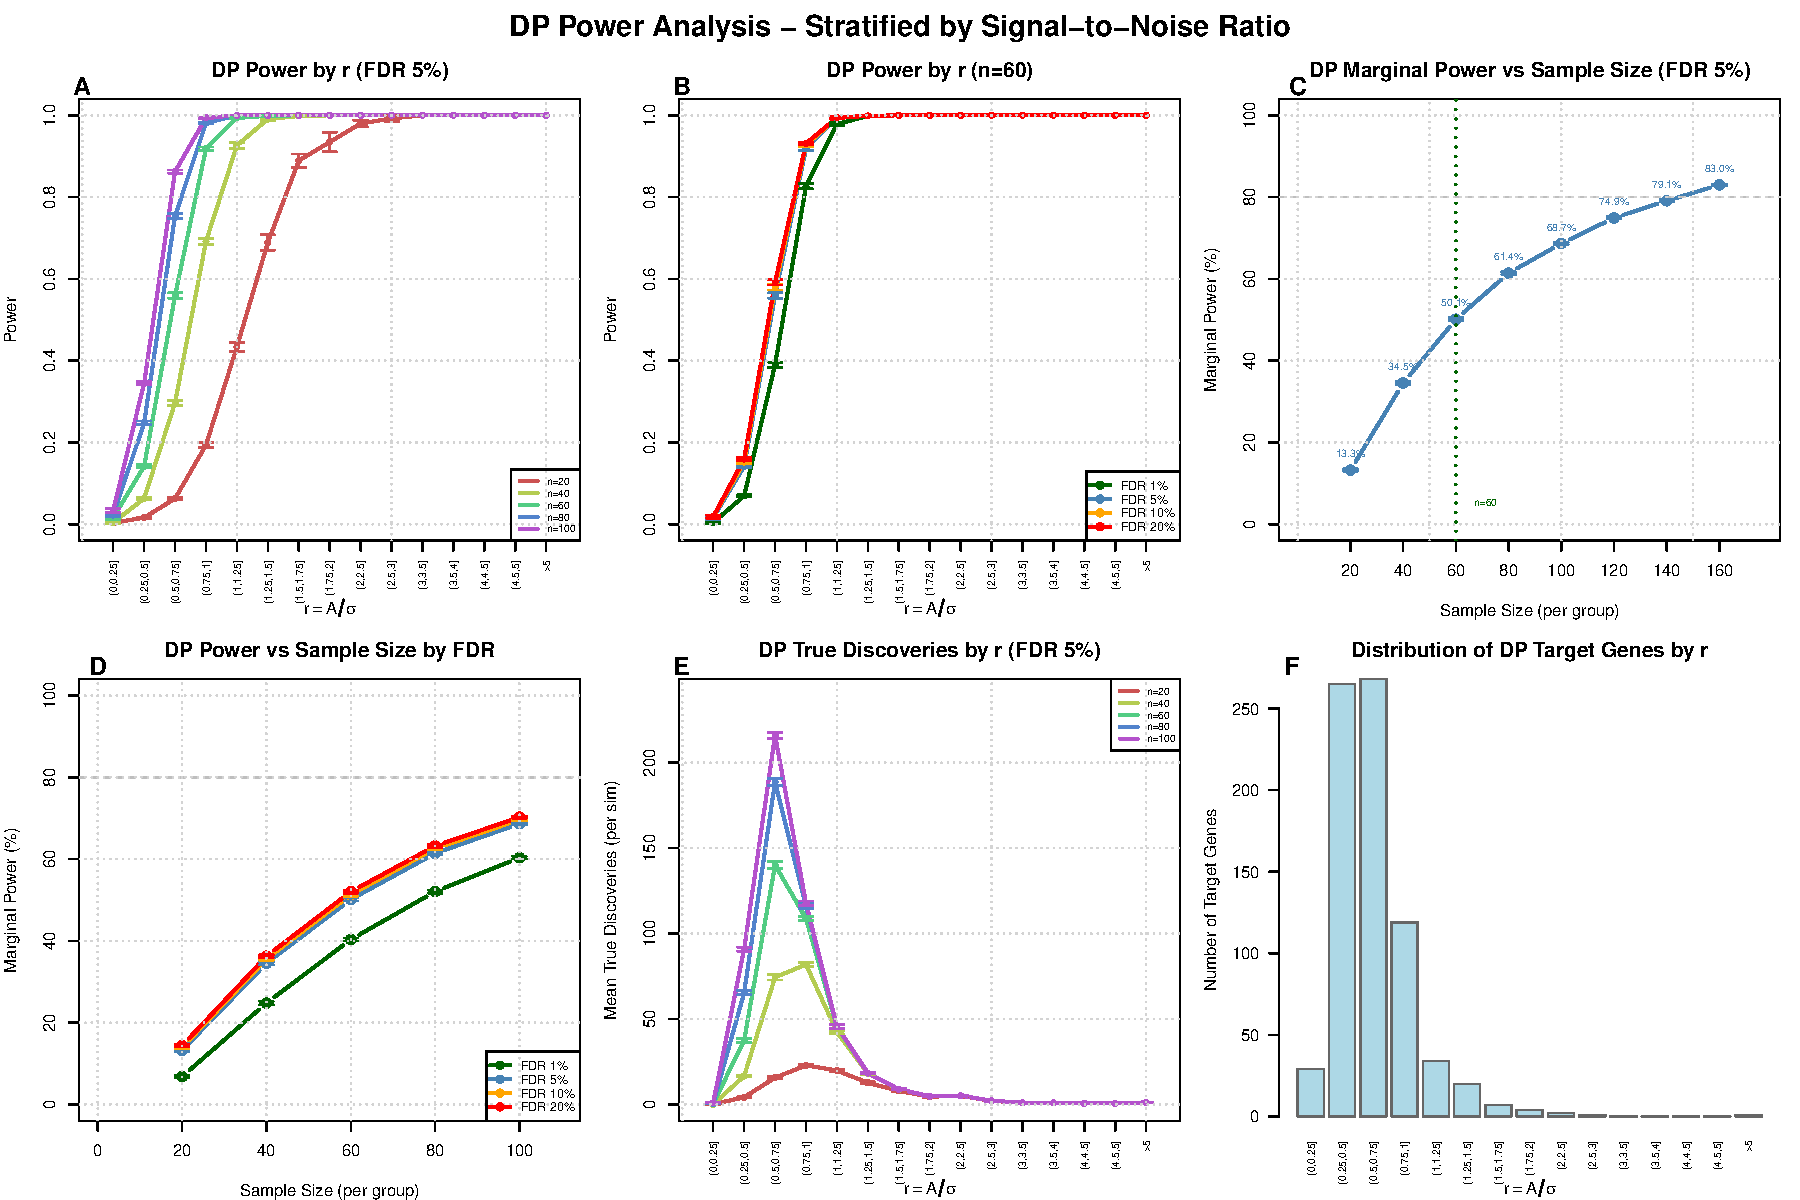
\includegraphics[width=\textwidth]{figures/dp_power.pdf}
\caption{DP power analysis ($\pm$6\,h phase shift). (B,D) show sensitivity to nominal FDR; (F) shows the empirical distribution of DP targets across $r$ strata. Panel layout otherwise matches Figure~\ref{fig:dr_power}.}
\label{fig:dp_power}
\end{figure}


\subsection{Phase Shift Sensitivity}

Power depends strongly on the magnitude of phase difference (Figure~\ref{fig:phase_shift_abdf}), serving as a sensitivity analysis for target definition based on phase shift magnitude $\Delta\phi$ (hours). Because a 12\,h shift is anti-phase and maximal, $\Delta\phi$ is naturally bounded to $[0,12]$\,h. At $n = 60$, overall (marginal) per-gene power increases from 0.2\% (0.5\,h shift) through 39.0\% (4\,h) to 52.6\% (8\,h), saturating beyond 8 hours (8\,h/12\,h power ratio $= 0.99$). Even at maximal (12\,h anti-phase) shifts, overall (marginal) per-gene power does not exceed 71.3\% ($n = 100$). Stratified analysis shows that genes with $r > 0.75$ achieve $\geq$80\% power for 4\,h shifts at $n = 60$ (Figure~\ref{fig:phase_shift_abdf}A). Full results are in Supplementary Section~S2.

\begin{figure}[H]
\centering
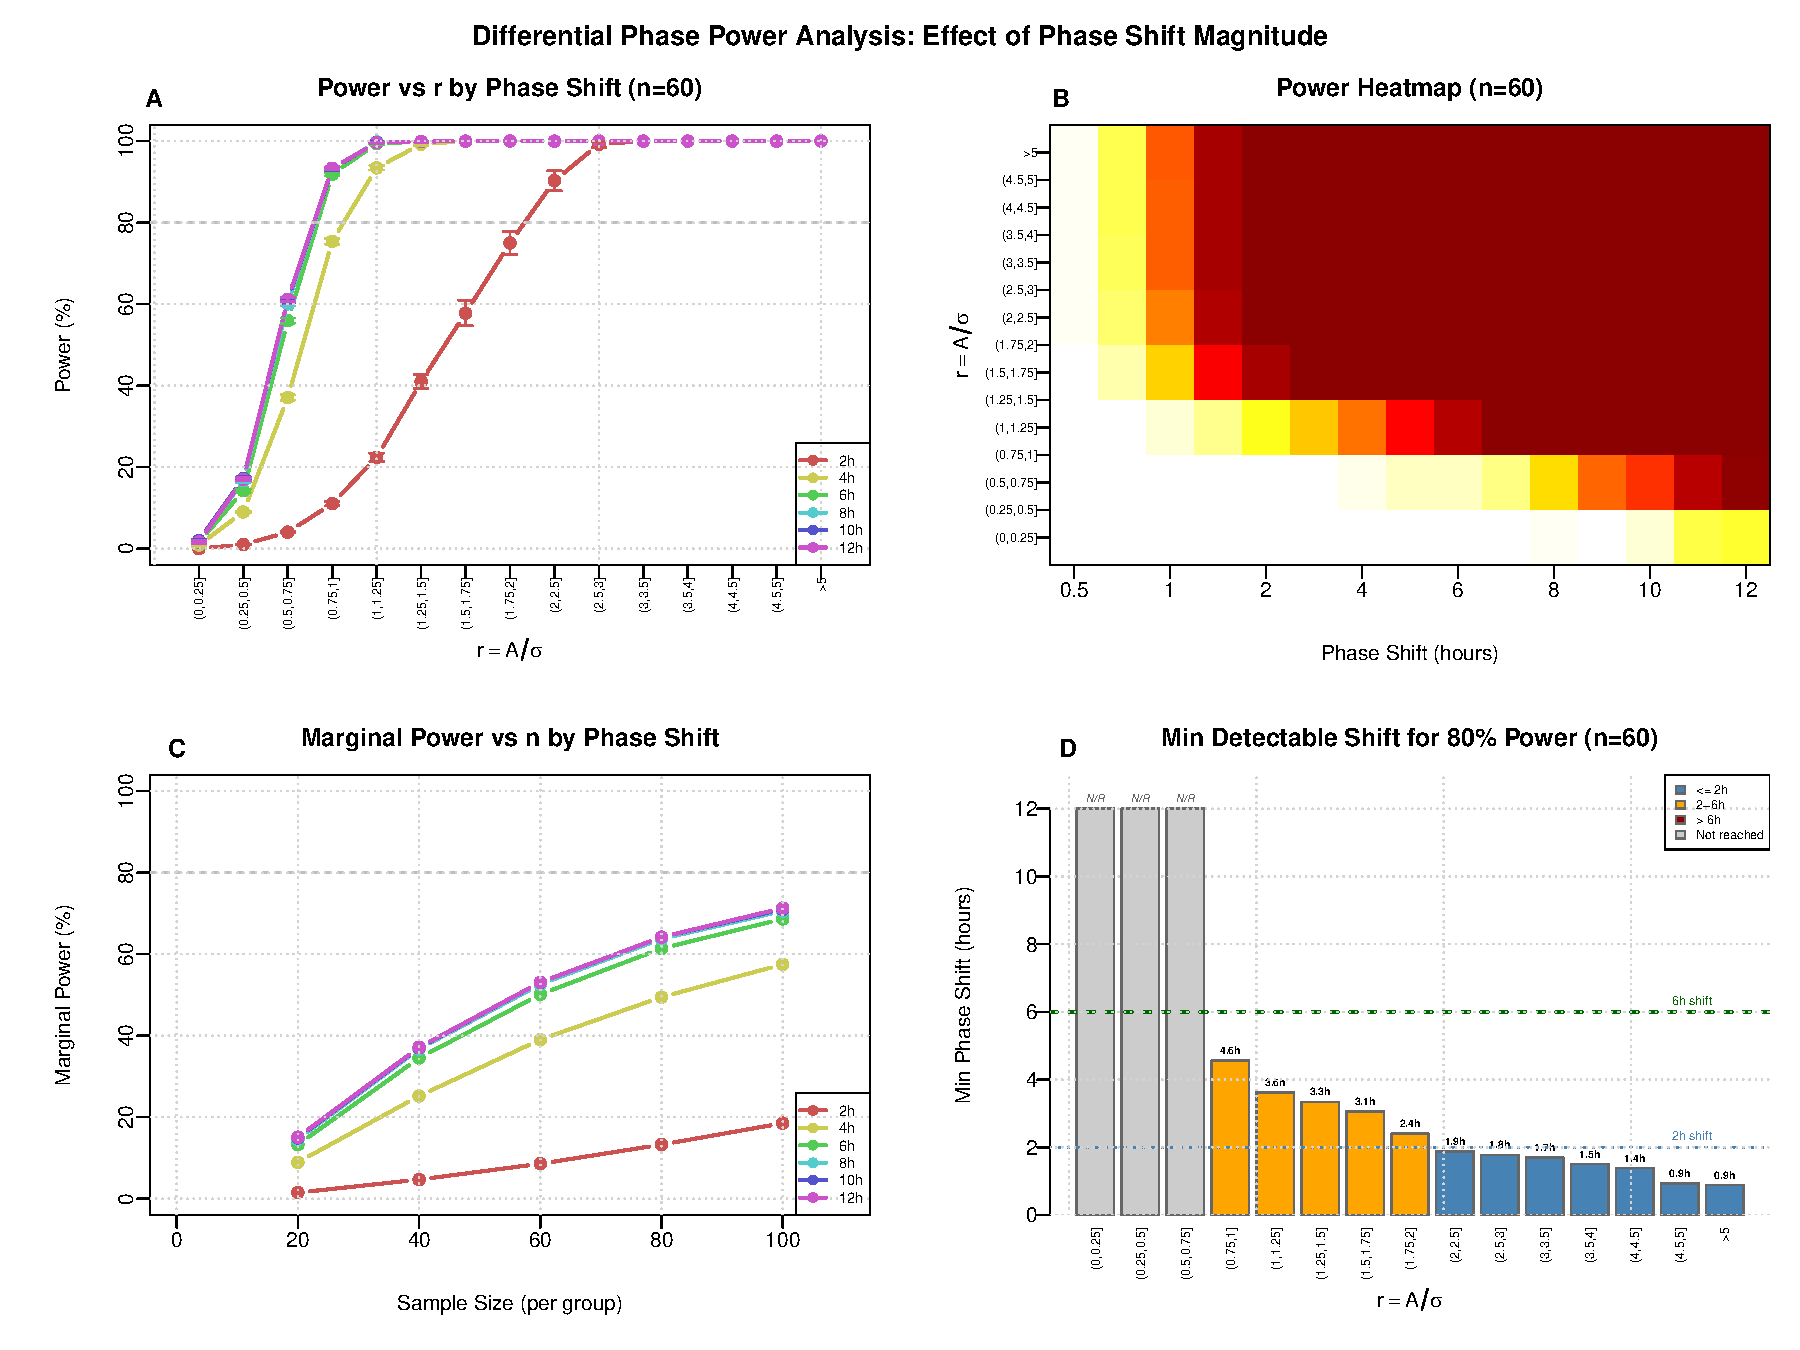
\includegraphics[width=\textwidth]{figures/phase_shift_abdf.pdf}
\caption{Phase shift sensitivity (5,000 genes, 50 simulations). (A) Power by $r$ stratum at $n=60$ across phase shifts. (B) Power heatmap ($r$ by phase shift). (C) Overall (marginal) per-gene power vs.\ sample size across phase shifts. (D) Minimum detectable phase shift by $r$ at $n=60$ (80\% power threshold).}
\label{fig:phase_shift_abdf}
\end{figure}

\subsection{Case Study: Comparing Detection Methods}

A key feature of \software{PowerSim}'s modular architecture is its ability to evaluate competing detection methods on identical simulated data, enabling objective comparisons of power and false discovery rate (FDR) to guide method selection. Methods such as \software{JTK\_CYCLE}, \software{RAIN}, and \software{MetaCycle} are designed for rhythmicity detection and do not perform hypothesis testing on individual circadian model parameters. We therefore focus on \software{DiffCircaPipeline} (DCP) and \software{CircaCompare} (CC), which conduct gene-level inference on individual circadian parameters.

DCP and CircaCompare differ in both scope and statistical approach. DCP provides a complete differential analysis pipeline: it tests DR (gain/loss of rhythmicity) via $\Delta R^2$ LRT, then tests DP among jointly rhythmic genes via constrained-MLE LRTs. CircaCompare tests per-parameter differences (DP and differential mesor) via Wald $t$-tests from per-gene NLS fits; it has no DR test equivalent because it lacks a $\Delta R^2$-type statistic for overall rhythm gain/loss. Thus for studies where DR is the primary question (e.g., identifying genes that lose rhythmicity in disease), DCP is the only available option.

For the shared test type (DP), we ran both methods on identical simulated datasets (Table~\ref{tab:method_comparison}; Figure~\ref{fig:method_comparison}). CircaCompare achieves 9--12 points higher DP power but at the cost of substantially inflated FDR (8.7--19.6\% vs.\ nominal 5\%; Figure~\ref{fig:method_comparison}B), meaning a considerable fraction of apparent DP discoveries are false positives. DCP maintains proper FDR control across all sample sizes. For differential mesor (DM, no true effects), both methods control Type~I error ($<0.002$). Stratified comparison (Supplementary Section~S4) shows the power gap is concentrated in moderate-$r$ strata ($0.5 < r < 1.5$); at high $r$ both methods converge to near-perfect power.

The computational cost difference is also substantial: DCP processes $G = 5{,}000$ genes in ${\sim}2$\,s per simulation (vectorized via \texttt{limma}), while CircaCompare requires ${\sim}150$\,s (${\sim}0.03$\,s/gene $\times$ NLS). For a full power analysis with 50 simulations $\times$ 5 sample sizes, DCP completes in ${\sim}8$ minutes vs.\ ${\sim}10$ hours for CircaCompare.

\begin{table}[H]
\centering
\small
\begin{tabular}{r|cc|cc}
\toprule
& \multicolumn{2}{c|}{Power} & \multicolumn{2}{c}{FDR} \\
$n$ & DCP & CC & DCP & CC \\
\midrule
20  & 13.2 & 23.5 & .063 & .196 \\
40  & 34.5 & 46.8 & .031 & .127 \\
60  & 50.1 & 61.8 & .024 & .100 \\
80  & 61.4 & 71.3 & .020 & .090 \\
100 & 68.6 & 77.5 & .023 & .087 \\
\bottomrule
\end{tabular}
\caption{Method comparison (CC = CircaCompare) for DP. Power (\%, FDR 5\% threshold) and empirical FDR. CircaCompare achieves higher DP power but inflates DP FDR to 9--20\%.}
\label{tab:method_comparison}
\end{table}

\begin{figure}[H]
\centering
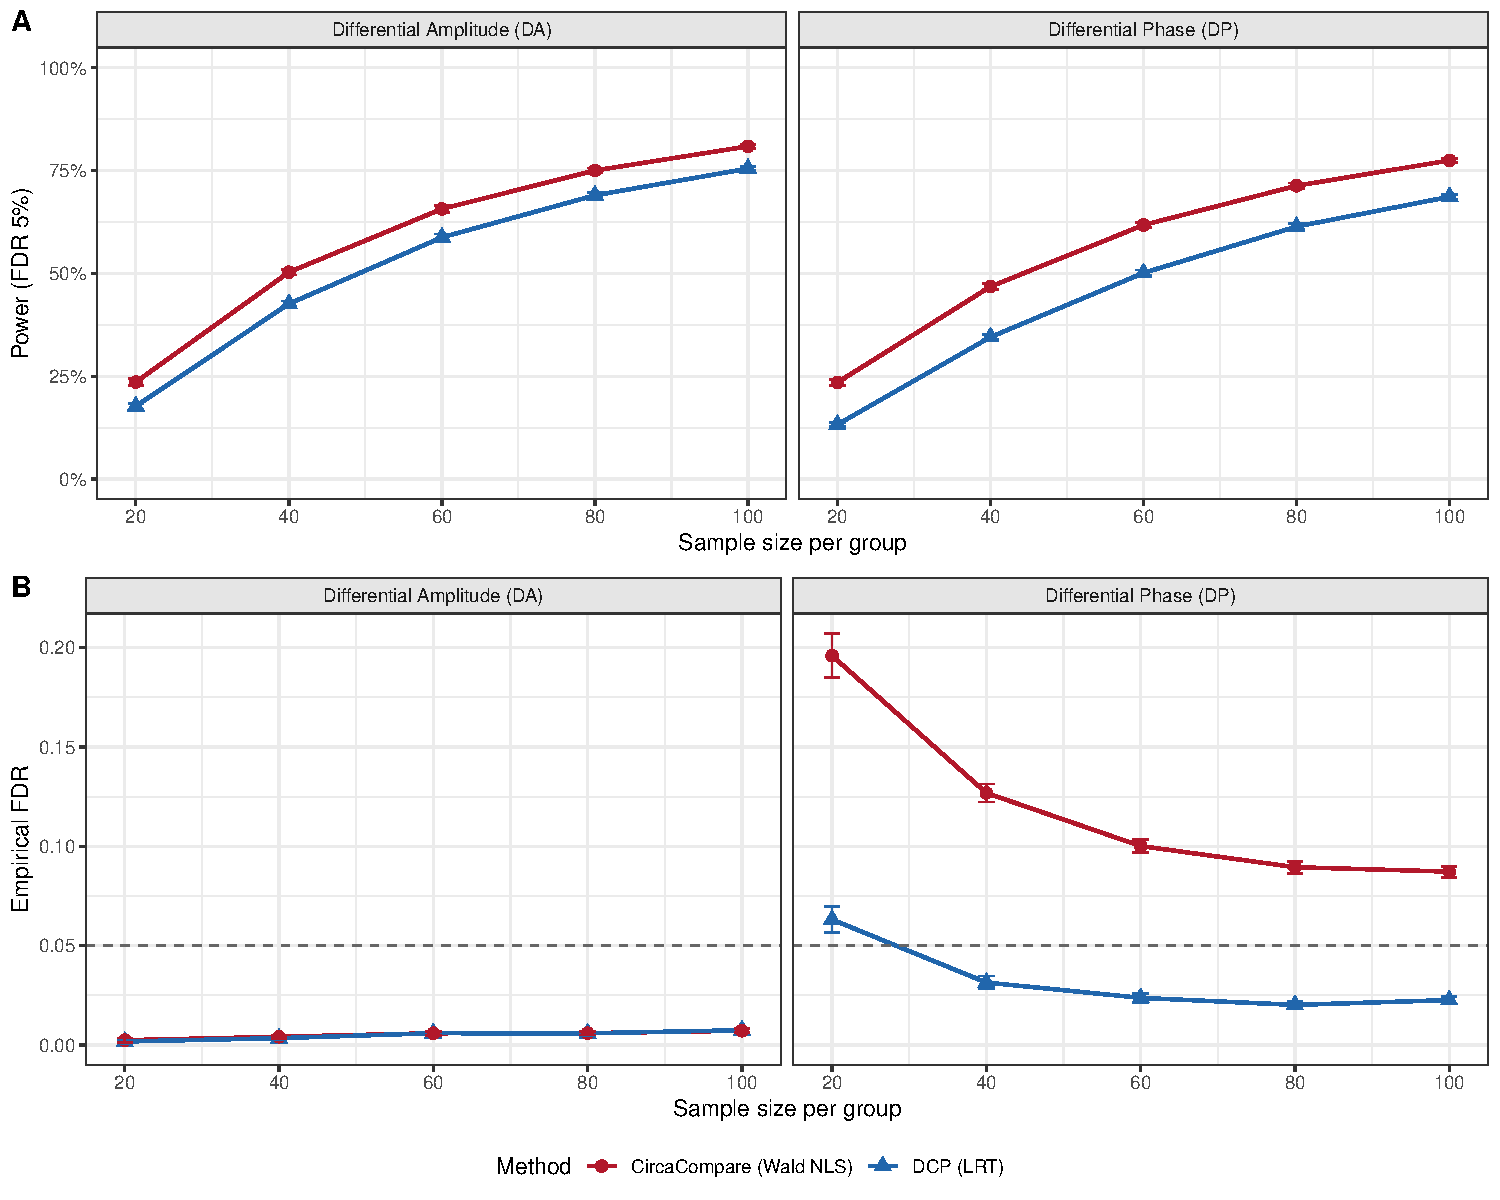
\includegraphics[width=\textwidth]{method_comparison/figures/method_comparison_combined.pdf}
\caption{Method comparison: DCP (LRT) vs.\ CircaCompare (Wald NLS) for DP. (A) Marginal power at FDR 5\%. CircaCompare achieves consistently higher power. (B) Empirical FDR. CircaCompare inflates FDR to 9--20\%, far above the nominal threshold (dashed line), while DCP maintains proper control. Error bars show $\pm$1.96 SE across 50 simulations.}
\label{fig:method_comparison}
\end{figure}

\subsection{Validation}

Framework validity was confirmed through four checks (details in Supplementary Section~S5):
(i) \emph{Type~I error control}: Under the complete null (no true differential genes), raw $p$-value rejection rates are near the nominal $\alpha = 0.05$ for DR (0.054--0.072) and DP (0.052--0.065). After BH correction, the false positive rate is 0.000 for all tests, confirming proper multiple testing control.
(ii) \emph{Power monotonicity}: Power increases monotonically with sample size for all tests and $r$-strata.
(iii) \emph{Effect size ordering}: Power increases monotonically with phase shift magnitude, saturating near 8\,h.
(iv) \emph{FDR calibration}: Empirical FDR is at or below nominal for DR (0.018--0.028) and DP (0.020--0.063), with slight inflation only at $n = 20$.

%% ====================================================================
\section{Discussion}
%% ====================================================================

% Our simulation study yields five principal findings.

% First, \textbf{DR detection is severely underpowered in human brain tissue}. Even at $n = 100$ per group, marginal DR power is only 30.5\%, driven by the low median effect size ($\tilde{r} = 0.556$) in post-mortem human brain. This is especially consequential for passive post-mortem studies, where samples are scarce, collection times are fixed, and design efficiency is reduced ($d \approx 0.24$ vs.\ $d = 0.5$ for active designs). Without simulation-based guidance, researchers risk committing years of tissue procurement to an underpowered study or missing the fact that targeted analysis of high-$r$ genes can yield reliable results with moderate sample sizes.

% Second, \textbf{stratified power analysis is essential}. Marginal power, which averages across genes with heterogeneous effect sizes, masks dramatic variation: high-$r$ genes ($r > 1.25$) are reliably detected at $n = 60$ ($\geq$83\% DR power) while low-$r$ genes ($r < 0.5$) remain below 5\% power even at $n = 100$. This parallels PROPER's finding for RNA-seq \cite{wu2015proper}; in circadian data the disparity is especially large because the $r$ distribution spans a 50-fold range.

% Third, \textbf{phase shift power saturates around 8 hours}. This reflects the geometric limit of cosine separation: for two cosines with identical $A$ and phase difference $\Delta\phi$, the squared amplitude of $y_1(t) - y_2(t)$ is proportional to $\sin^2(\pi\Delta\phi/\tau)$, which plateaus for $\Delta\phi > \tau/3 \approx 8$\,h.

% Fourth, \textbf{the case study comparing DCP and CircaCompare illustrates how \software{PowerSim} can guide method selection}. The two methods occupy complementary niches. DCP is the only tool providing a DR test for overall gain/loss of rhythmicity, making it indispensable when DR is the primary scientific question. For the shared test type (DP), CircaCompare offers 9--12 percentage points higher power but at the cost of inflated DP FDR (9--20\% vs.\ nominal 5\%) and ${\sim}75\times$ longer computation time. When the effective true discovery rate is adjusted for false positives, $\text{Power}_{\text{adj}} = \text{Power} \times (1 - \widehat{\text{FDR}})$, the DP gap narrows substantially (e.g., at $n = 60$: DCP $50.1\% \times 0.976 = 48.9\%$ vs.\ CC $61.8\% \times 0.900 = 55.6\%$). For DP, DCP is preferred in discovery studies where FDR control is critical, while CircaCompare may be considered when the power gain outweighs the inflation risk and findings will be independently validated. The computational difference is also practically relevant: a full power analysis across 50 simulations and 5 sample sizes completes in ${\sim}8$ minutes with DCP versus ${\sim}10$ hours with CircaCompare, making DCP far more suitable for exploratory analyses involving many scenarios. More broadly, this case study demonstrates how \software{PowerSim}'s pluggable architecture enables evidence-based method choices by running competing methods on identical simulated data.

% \paragraph{Practical recommendations.} For DR in human brain tissue: $n \geq 80$ for modest overall (marginal) per-gene power; targeted analyses of high-$r$ genes can succeed with $n = 40$--60. For DP ($\pm$6\,h shifts): $n = 60$ achieves 50\% overall (marginal) per-gene power. These recommendations are specific to human post-mortem brain, which has among the lowest circadian effect sizes of any tissue \cite{zong2023circapower} and therefore represents a conservative design baseline. For actively-designed mouse studies, where core-gene $r$ values are typically 3--10$\times$ higher ($r \approx 2$--$6$; CircaPower Table~1), substantially smaller sample sizes would suffice. Active designs also benefit from a higher design factor ($d = 0.5$ vs.\ ${\sim}0.24$ for passive), further reducing sample requirements. In all cases, we recommend reporting stratified alongside overall (marginal) per-gene power, as the latter can be misleading when $r$ is heterogeneous and can obscure actionable design guidance.

% \paragraph{Why stratified power matters.} Marginal power averages over the full distribution of $r$ and is dominated by the large mass of low-$r$ genes in human brain, leading to uniformly low averages even when a subset of strong rhythms is well powered. Stratified power makes this heterogeneity explicit by reporting power within $r$-bins, showing which effect sizes are detectable at feasible $n$. This framing supports targeted study design: investigators can choose sample sizes based on the effect-size range that is biologically meaningful rather than a single marginal average.

% \paragraph{Limitations.} Current limitations include: (i) independent marginal resampling of $\mu_g$, $\sigma_g$, and $A_g$ (ignoring potential correlations across genes; joint resampling of per-gene parameter tuples would preserve the empirical correlation structure); (ii) passive design results are specific to the pilot data's time-of-day distribution (different tissues or cohorts may have different $F_{\text{TOD}}$ and hence different $d$); (iii) computational cost of CircaCompare (${\sim}150$\,s per simulation vs.\ ${\sim}2$\,s for DCP) limits feasible $N_{\text{sim}}$; (iv) the cosinor model assumes sinusoidal waveforms, which may not capture asymmetric or bimodal expression patterns in some genes; and (v) BH control assumes independence or PRDS across genes, whereas gene--gene correlations may affect calibration in practice.

% A further limitation is that differential gene types are modeled as mutually exclusive: each gene is assigned to exactly one of DR or DP, and compound changes (e.g., a gene that simultaneously shifts phase and loses rhythmicity, as commonly observed in aging or neuropsychiatric disease) are not simulated. In real transcriptomes, circadian disruption often manifests as correlated multi-parameter changes rather than isolated single-parameter shifts. However, simulating each differential type in isolation is the standard approach in power analysis for multi-parameter tests, for the same reason that DE power analysis evaluates fold-changes in isolation: it allows clean, interpretable power curves for each test type and avoids confounding from compound effects that would make it impossible to attribute detection to a specific test. The one-at-a-time design is therefore appropriate for the primary goal of guiding study design, where investigators typically need to know the power for a specific hypothesis (e.g., ``how many subjects to detect phase-shifted genes?'') rather than the power under a complex joint model. Future work could extend the framework to compound-type genes to evaluate robustness of test specificity under realistic multi-parameter disruption.

% \paragraph{Software availability.} \software{PowerSim} is available as an open-source R framework with a PROPER-style configuration system. An end-to-end pipeline (\texttt{examples/run\_pipeline.R}) reproduces all results in this paper, and a validation suite (\texttt{examples/run\_validation.R}) implements the checks described in Section~3.6.

\section*{Acknowledgments}

This work builds on \software{CircaPower} \cite{zong2023circapower}, \software{PROPER} \cite{wu2015proper}, \software{DiffCircaPipeline} \cite{xue2023diffcircapipeline}, and \software{CircaCompare} \cite{parsons2020circacompare}.

\bibliographystyle{plain}
\bibliography{references}

\end{document}
